 
% rtlu.discrete
 	\begin{center}
	\addtolength{\leftskip}{-4cm}\addtolength{\rightskip}{-4cm}

\begin{tabular}{|c|c|cc|}
\hline
\multicolumn{4}{|c|}{\textbf{\underline{\textbf{\underline{data$brothersSisters}}}}}\\

\multicolumn{4}{|c|}{Discrete(6) \hfill N=156 ; NA=0 (0\%)}\\
\hline
 \textbf{Frequency} & \textbf{Summary} & \textbf{Boxplot} & \textbf{Histogram} \\

 \begin{tabular}{@{}l@{ : }cl@{}}

  0 & 51 & (32.69\%) \\

  1 & 67 & (42.95\%) \\

  2 & 28 & (17.95\%) \\

  3 & 6 & (3.85\%) \\

  4 & 3 & (1.92\%) \\

  5 & 1 & (0.64\%) \\

 \end{tabular}
 & \begin{tabular}{@{}l@{ : }c@{}}

          Mean    & 1.013 \\

          Var.    & 0.942 \\

          SD      & 0.97 \\
\hline
          Min.    & 0 \\

          Q1      & 0 \\

          Median  & 1 \\

          Q3      & 1 \\

          Max.    & 5 \\

 \end{tabular}
 & \parbox{3cm}{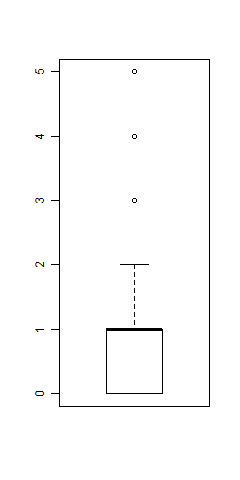
\includegraphics[width=3cm]{graphUniv6/V-boxplot.png}}
 & \parbox{7cm}{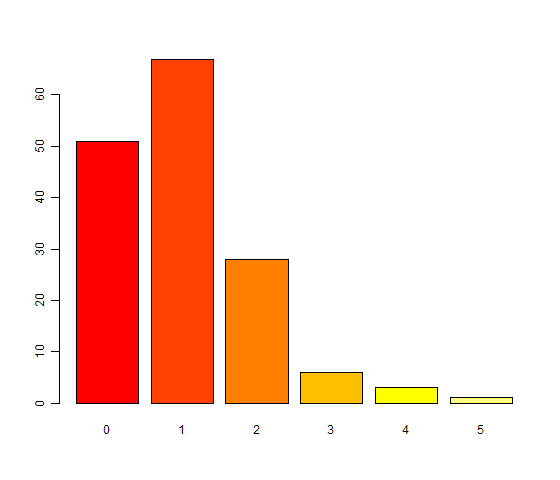
\includegraphics[width=7cm]{graphUniv6/V-barplot.png}}
 \\
\hline
\end{tabular}
\end{center} 
